\section{Results}
\subsection{Single-Task Classifiers}
\paragraph*{Naive Bayes}
We ran Naive Bayes and logistic regression on all 6 tasks independently and computed accuracy, precision, recall and the F1-measure of each classifier. 

We first trained and run Naive Bayes using the different thresholds. Figure \ref{fig:naivebayes} gives all the results for the Naive Bayes classifier. As expected, we found that the Naive Bayes classifier can not profit from multi-bit features, as they clearly violate the independence assumption. In the task lawnmower, where 95\% of all submissions solve the large testcase, the multi-bit versions perform significantly worse than the median- and mean-versions. In the other tasks the differences were smaller, so we used the median threshold for further experiments, as it performed best on average.

%
\begin{figure}
    \centering
    \setlength{\tabcolsep}{0.0130\linewidth}
    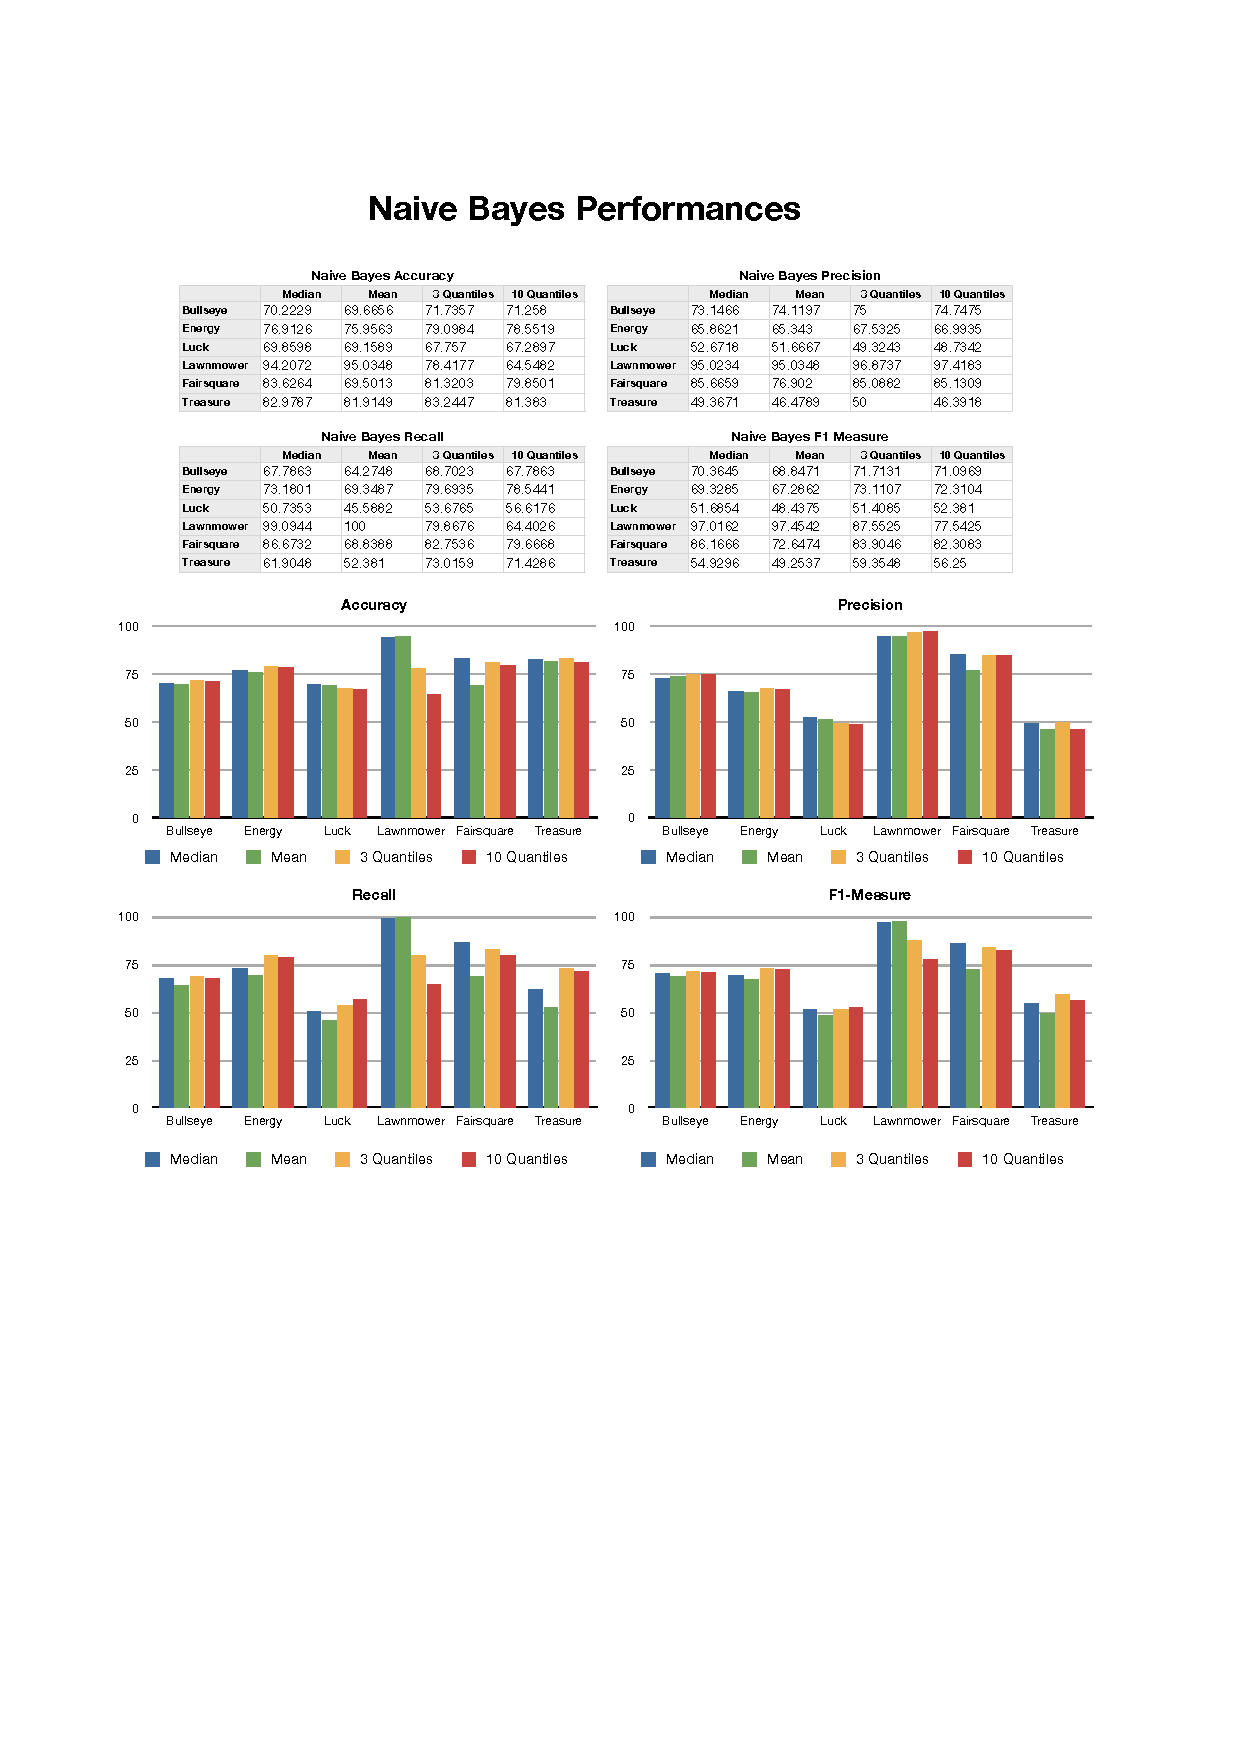
\includegraphics[width=\linewidth]{figures/NaiveBayes}
    \caption{Performance of the Naive Bayes classifier.%
      \label{fig:naivebayes}}
\end{figure}

\paragraph*{Logistic Regression}
Figre \ref{fig:logisticregression} summarizes the result on logistic regression for different regularization parameters $\lambda \in [10^{-2}, 10^{-3}, 10^{-4}, 10^{-5}$. We used the quartile-thresholds for this experiment, where each integer feature is represented using 3 bits. For the four easier tasks the results were almost identical. Only in the two hard tasks \emph{Luck} and \emph{Treasure} the choice of $\lambda = 10^{-3}$ works best. So we used this value in the later comparison.

%
\begin{figure}
    \centering
    \setlength{\tabcolsep}{0.0130\linewidth}
    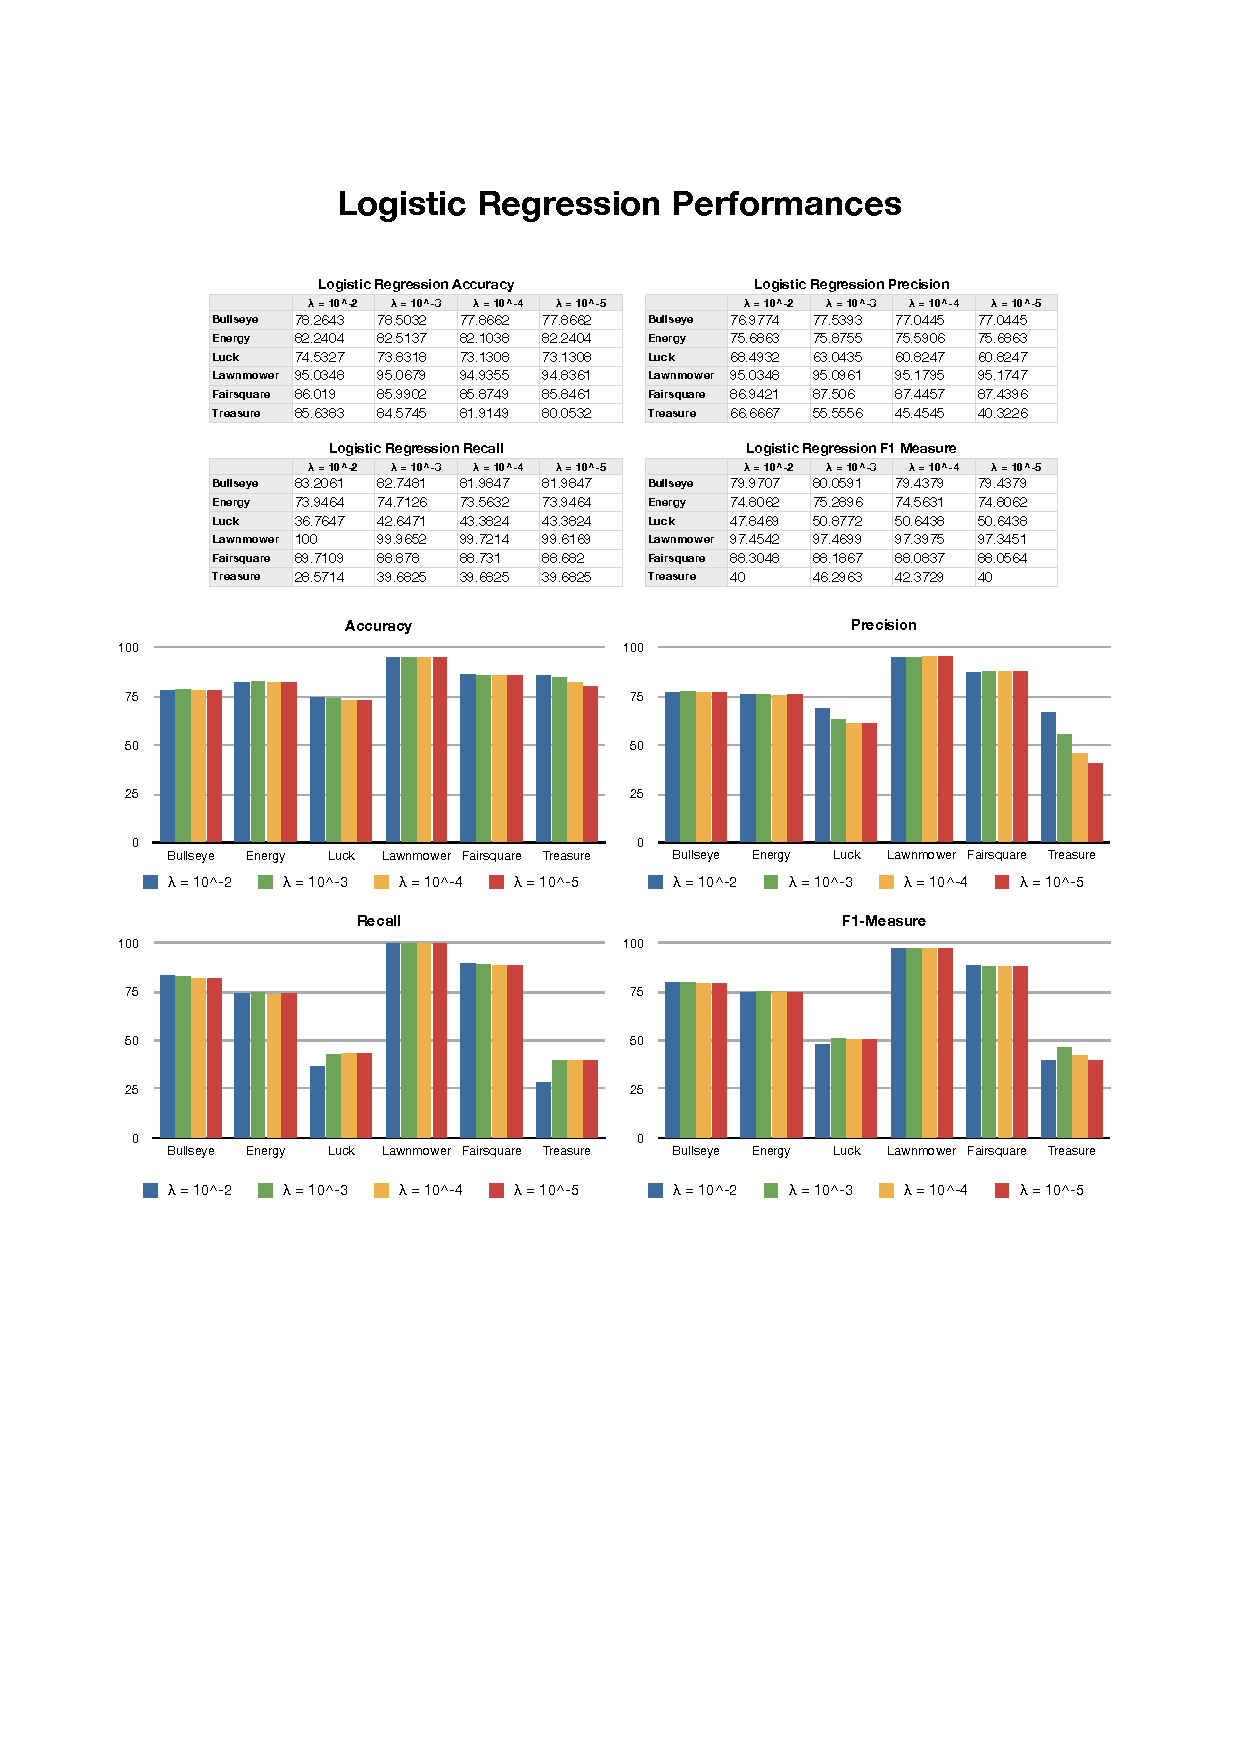
\includegraphics[width=\linewidth]{figures/LogisticRegression}
    \caption{Performance of the logistic regression classifier.%
      \label{fig:logisticregression}}
\end{figure}

\paragraph*{Single-Task Comparison}
Next, we compared the following four classifiers:

\begin{itemize}
\item Naive Bayes using the median as threshold and only the first 5 features (code length in bytes and lines, number of includes, number of loops and number of variables)
\item Naive Bayes using the median as threshold and all 35 features
\item Logistic regression using a single bit per feature from the median threshold
\item Logistic regression using three bits per feature from the quartile thresholds
\end{itemize}

The results are listed in Figure \ref{fig:singletask}. We can see that the three-bit logistic regression outperforms the Naive Bayes in the four easier tasks, but falls behind it in the four harder tasks.

%
\begin{figure}
    \centering
    \setlength{\tabcolsep}{0.0130\linewidth}
    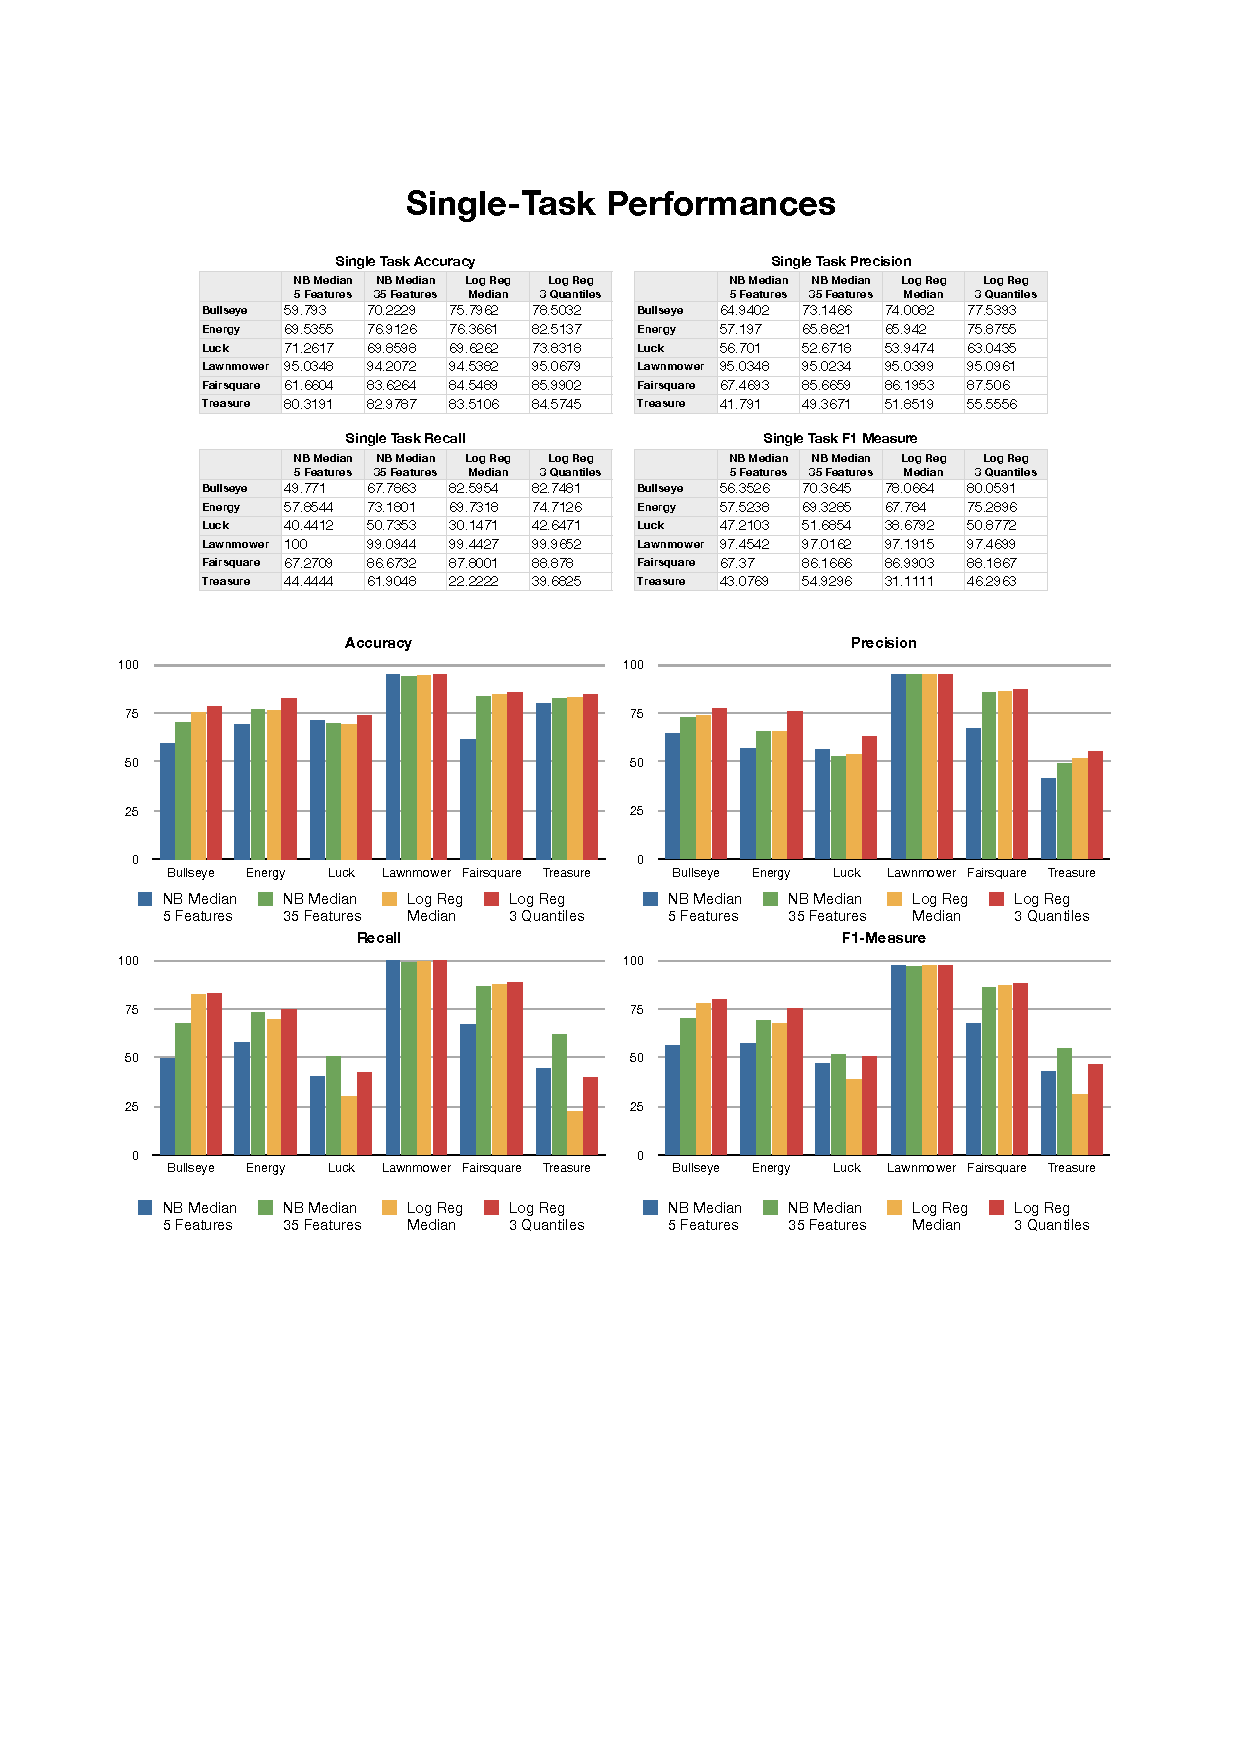
\includegraphics[width=\linewidth]{figures/SingleTask}
    \caption{Comparison of the various single-task classifiers.%
      \label{fig:singletask}}
\end{figure}


\subsection{Multi-Task Classifiers}


%
\begin{figure}
    \centering
    \setlength{\tabcolsep}{0.0130\linewidth}
    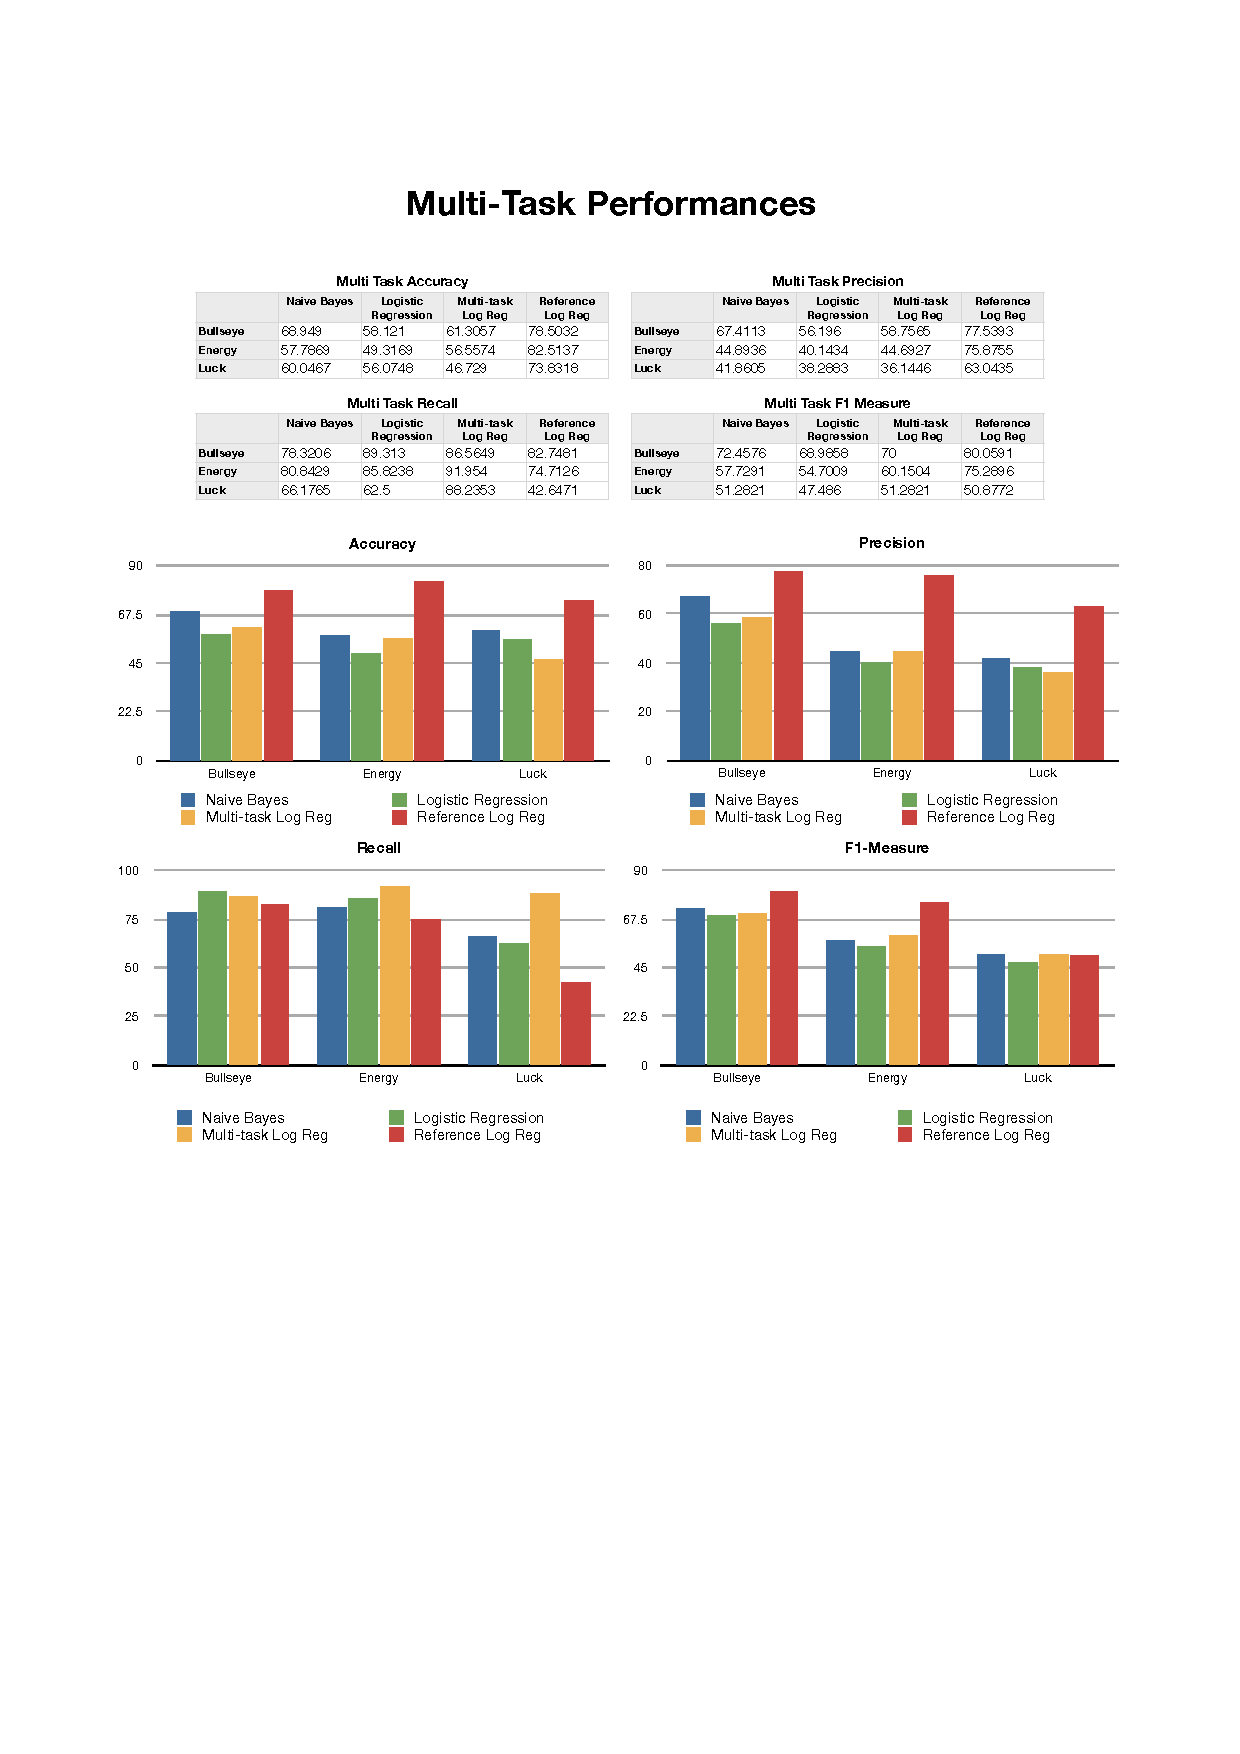
\includegraphics[width=\linewidth]{figures/MultiTask}
    \caption{Comparison of the various multi-task classifiers.%
      \label{fig:multitask}}
\end{figure}


All the data, code and results of our experiments can be found on our 
\href{https://github.com/johnnyyan/515project}{GitHub-repository (link)}.

